\chapter{Realizability of Polygonal Linkages with Fixed Orientation\label{chapter:polygonalLinkage}}

We begin the chapter with describing several gadgets that translates the associated graph $A(\Phi)$ of a P3SAT boolean formula.  
These gadgets will be used together to form a special hexagonal tiling that behaves in a similar nature to the logic engine that encoded a NAE3SAT instance of Chapter \ref{chapter:logicEngine} but instead encodes a Planar 3-SAT and its associated graph.
Together the gadgets will form what is called the auxilary construction.
A hexagonal tiling and several gadgets enclosed in a frame (a frame that is conceptually similar to the frame found in a logic engine) would then be used to prove the following theorem:
\begin{thm}\label{thm:hinge2}
It is strongly NP-hard to decide whether a polygonal linkage whose hinge graph is a \textbf{tree} can be realized with counter-clockwise orientation.
\end{thm}
Our proof is a reduction from P3SAT.
Given an instance $\Phi$ of P3SAT with $n$ variables and $m$ clauses and its associated graph $A(\Phi)$, we construct a simply connected polygonal linkage $(\PP,H)$, of polynomial size in $n$ and $m$, such that $\Phi$ is satisfiable if and only if $(\PP,H)$ admits a realization with fixed orientation. 

We construct a polygonal linkage in two main steps: first, we construct an auxiliary structure where some of the polygons have fixed position in the plane (called \emph{obstacles}), while other polygons are flexible, and each flexible polygon is hinged to an obstacle. 
Second, we modify the auxiliary construction into a polygonal linkage by allowing the obstacles to move freely, and by adding new polygons and hinges as well as an exterior \emph{frame} that holds the obstacle polygons in place.
All polygons in our constructions are regular hexagons or long, skinny rhombi.
In Chapter \ref{chp:disk} we can ``simulate'' these shapes with disk arrangements to show related results.

Storer, Tamassia, and Tollis showed that if $G=(V,E)$ is planar, it can be embedded in an $\vert V \vert \times \vert V \vert$ grid with $S(G)=2.4\vert V\vert + 4$ bends \cite{storer1984minimal,tamassia1987efficient}.
Note that this result implies that a planar graph can be embedded in a grid of size $S(G) \times S(G)$; and this allows $S(G)$ to act as a fundamental polynomial problems with planar graphs defined in a embedding in a grid.
We can define a \textit{bend polynomial}, $s(n,m)$ that will be used to construct our gadgets which will be used to prove Theorem \ref{thm:hinge2}.
For our constructions, our bend polynomial can be any polynomial strictly greater than $S(G)$, e.g.:
$$6 (n+m) + 4.$$
The table below is a glossary of formulas that are used to throughout this chapter.
It will serve as a useful reference for the reader.
$$
\begin{array}{|rcl|}
\hline
z(n,m)		&=& 4 s(n,m)\\\hline
J_h (z) 	&=& 6z(n,m)+1 = 24s(n,m)+1 \\\hline
J_d (z) 	&=& 4z(n,m)+1												= 16s(n,m)+1  			\\\hline
N(n,m)		&=& \frac{5t-1}{2}											= \frac{5s^\kappa-1}{2}	\\\hline
t(n,m)		&=& s^\kappa																		\\\hline
H(n,m) 		&=&  (12s+1)  (5t-1)  \sqrt{3} + 12s \lr{\sqrt{3}+ \frac{1}{250t-50}}				\\\hline
&&x - \frac{x^3}{3}\leq\tan^{-1}x\leq x \qquad	 0< x < 1\\\hline
&&\leq x - \frac{x^3}{6}\sin x \leq x \quad\qquad 0< x < 1\\\hline
&&\cos x \leq 1-\frac{x^2}{2} \qquad\qquad 0< x < 1\\\hline
&&\sec x \leq 1+\frac{x^2}{2} \qquad\qquad 0< x < 1\\\hline
\end{array}
$$
% blhlakjdlaj
% $$
% \begin{array}{|rclcrcl|}
% \hline
% z(n,m)		&=& 4 s(n,m)																  		&&r&c&l\\\hline
% J_h (z) 	&=& 6z(n,m)+1												= 24s(n,m)+1  			&&r&c&l\\\hline
% J_d (z) 	&=& 4z(n,m)+1												= 16s(n,m)+1  			&&r&c&l\\\hline
% N(n,m)		&=& \frac{5t-1}{2}											= \frac{5s^\kappa-1}{2}	&&r&c&l\\\hline
% t(n,m)		&=& s^\kappa																		&&r&c&l\\\hline
% H(n,m) 		&=&  (12s+1)  (5t-1)  \sqrt{3} + 12s \lr{\sqrt{3}+ \frac{1}{250t-50}}				&&r&c&l\\\hline
% 			&& 	x - \frac{x^3}{3}\leq\tan^{-1}x\leq x											&&&&0< x < 1 \\\hline
% \sin x 		&& x 																				&&r&c&l\\\hline
% \cos x 		&& 1-\frac{x^2}{2}																	&&r&c&l\\\hline
% \sec x 		&& 1-\frac{x^2}{2}																	&&r&c&l\\\hline
% \end{array}
% $$
The formula $t(n,m)=s^\kappa$ has an exponent $\kappa$ which is a sufficiently large integer that is chosen later on so that all arguments in this chapter are satisfied.
The trigonmetric functions in the table above each are expressed as either the first term or the first and second term of their Maclaurin Series expansion.

\paragraph{Modifying the Associated Graph of a P3SAT.}

Given an instance of P3SAT boolean formula $\Phi$ of $n$ variables and $m$ clauses with associated graph $A(\Phi)$, we construct a finite \textit{honeycomb} grid $H_{A \lr{\Phi}}$ of regular hexagons over the plane centered at origin.
We modify the associated graph drawing $A\lr{\Phi}$ by overlaying it onto a honeycomb in the following way:

\begin{enumerate}
%variables represent cycles of 2m 
\item \textbf{Variable:} A vertex representing a variable shall encompass a consecutive set of hexagons along a horizontal line in the honeycomb (see Figure \ref{fig:VariablesExample.pdf}).

\begin{minipage}{\linewidth}
\begin{center}
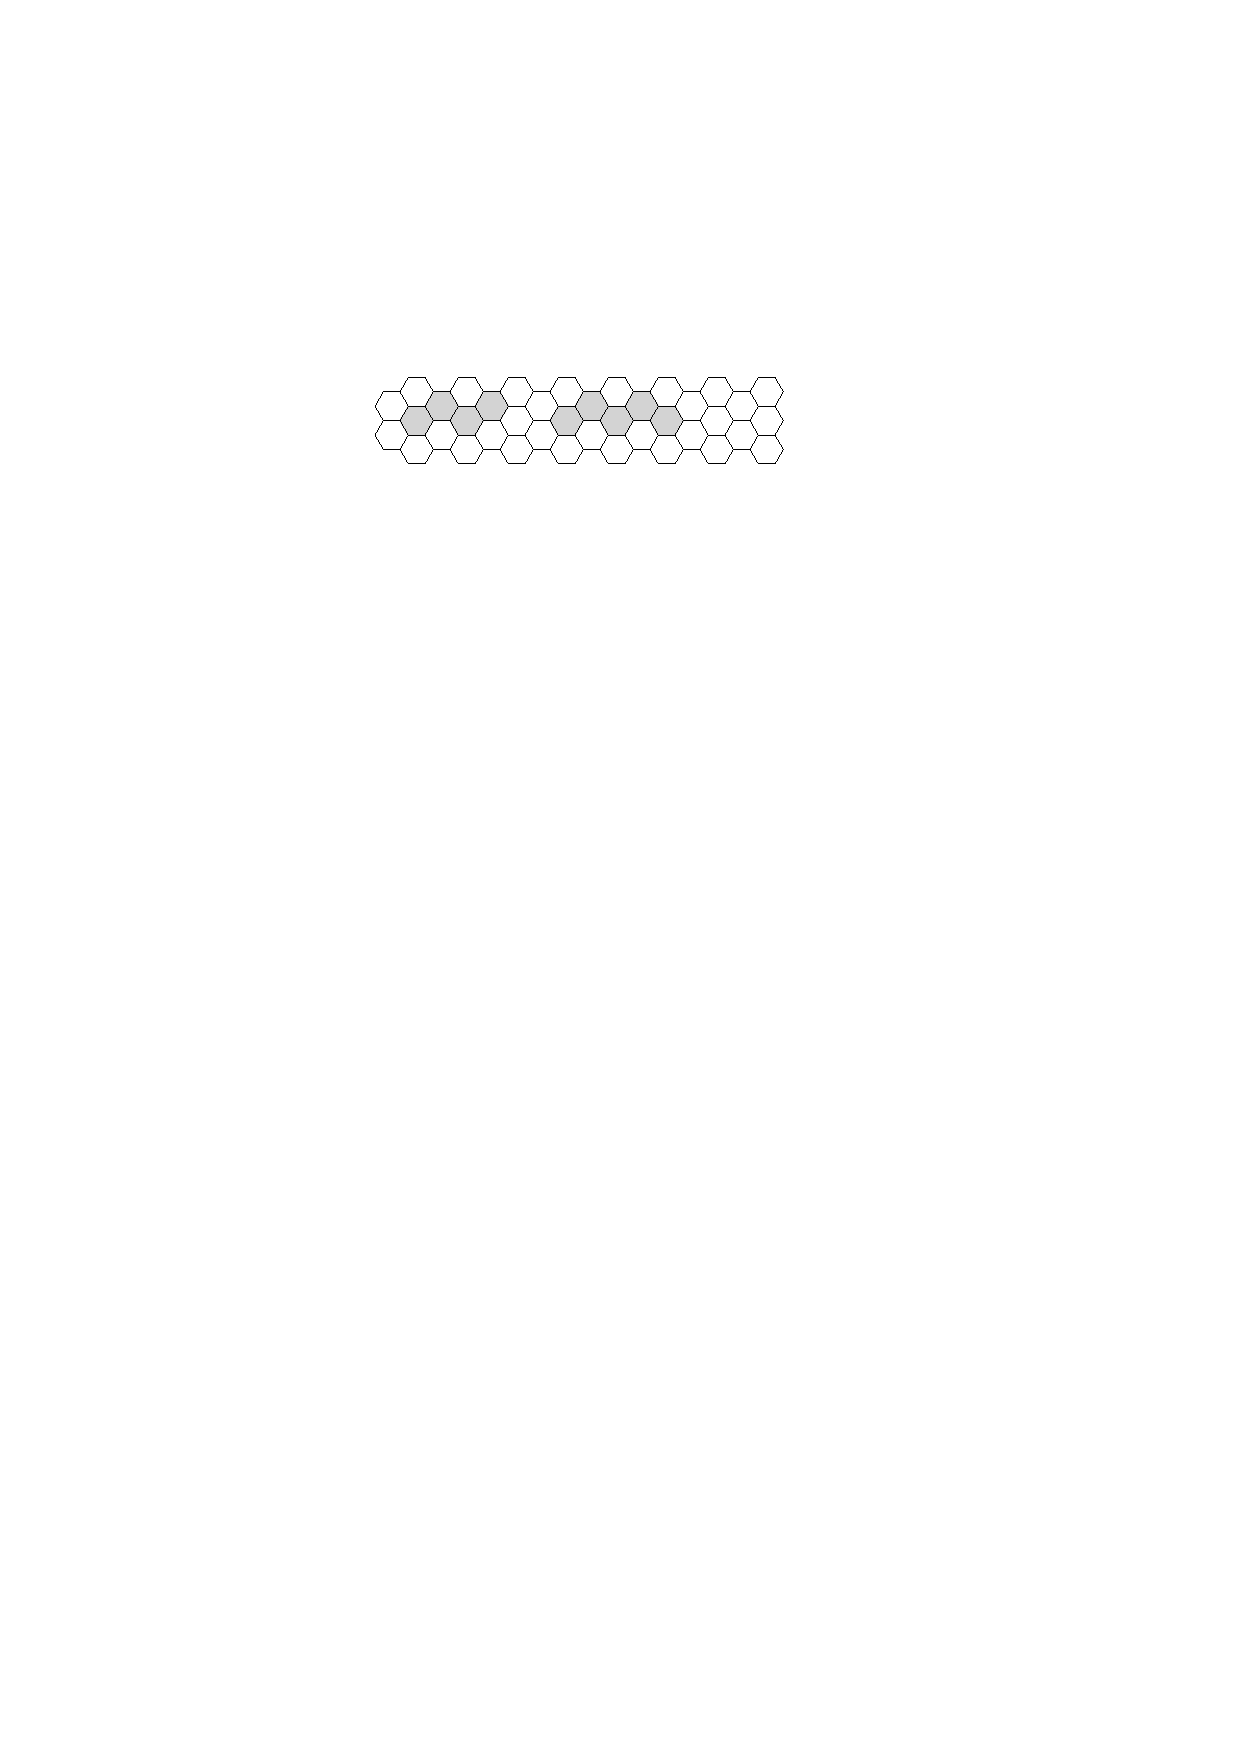
\includegraphics[width=.75\textwidth]{graphics/VariablesExample.pdf}
\captionof{figure}{The four shaded groups of horizontally adjacent hexagons represent four distinct variables from a boolean formula in the honeycomb.}\label{fig:VariablesExample.pdf}
\end{center}
\end{minipage}

Let $D = \max_{v \in V} \deg(v)$ where $V$ is the set of vertices of $A(\Phi)$.
Every variable vertex $v$  must encompass at least $2 \cdot \deg(v)$ consecutive hexagons but can encompass up to $2 \cdot D$ consecutive hexagons.
\item \textbf{Clause:} A vertex representing a clause shall be a vertex of a hexagon in the honeycomb.
\item \textbf{Edge:} Edges of the associated graph $A(\Phi)$ are paths between the variable $x_i$ and clause $C_j$.  An edge $\left\lbrace x_i, C_j \right\rbrace$ of the associated graph is pariwise edge disjoint. 
The edges of the drawing shall traverse the edges of hexagons in a vertically or horizontally zigzagging manner (see Figure \ref{fig:HoneyCombAssociatedGraphSmall}) in the honeycomb from the literal to the corresponding clause. 
Edges traverse a hexagon in two edges vertically, three edges horizontally.  
The vertical zigzagging edge segments traverse the left or right sides of a hexagon(s).
The horizontal zigzagging edge segments traverse the top or bottom halves of a hexagon(s).
When the edge transisitions from a vertical to horizontal traversal, the edge traverses in over 4 edges about the hexagon.
The length of the edges are bounded above by $6 \cdot \lr{\ell_1 \lr{x_i,C_j} + D}$ where $\ell_1$ is the $L_1$ norm. 
\end{enumerate}

Figure \ref{fig:HoneyCombAssociatedGraphSmall} illustrates an associated graph of a P3SAT overlayed on a honeycomb.
This type of construction emulates an \textit{orthoganal drawing} over a hexagonal grid; an orthoganal drawing where edges are drawn with alternating vertical and horizontal line segments.
Let the region in which the construction lies in be a regular hexagon region with polynomial side length $s(n,m)$. 

\begin{minipage}{\linewidth}
\begin{center}
\includegraphics[width=.9\textwidth]{graphics/HoneyCombAssociatedGraphSideBySide.pdf}
\captionof{figure}{
(a) This is an instance of an associated graph for a P3SAT overlayed onto a honeycomb grid and placed into a regular hexagonal region.
This honeycomb graph could correspond to Boolean formula $\lr{\lnot x_1 \lor \lnot x_2 \lor x_4} \land \lr{x_2 \lor \lnot x_3 \lor x_4} \land \lr{x_1 \lor \lnot x_3 \lor \lnot x_4}$. (b) This is the same instance as (a) shown without the hexagonal region.
}\label{fig:HoneyCombAssociatedGraphSmall}
\end{center}
\end{minipage}

The honeycomb construction will act as preliminary concept that will be refined further in the Auxilary Contruction.